%% ****** Start of file apstemplate.tex ****** %
%%
%%
%%   This file is part of the APS files in the REVTeX 4 distribution.
%%   Version 4.1r of REVTeX, August 2010
%%
%%
%%   Copyright (c) 2001, 2009, 2010 The American Physical Society.
%%
%%   See the REVTeX 4 README file for restrictions and more information.
%%
%
% This is a template for producing manuscripts for use with REVTEX 4.0
% Copy this file to another name and then work on that file.
% That way, you always have this original template file to use.
%
% Group addresses by affiliation; use superscriptaddress for long
% author lists, or if there are many overlapping affiliations.
% For Phys. Rev. appearance, change preprint to twocolumn.
% Choose pra, prb, prc, prd, pre, prl, prstab, prstper, or rmp for journal
%  Add 'draft' option to mark overfull boxes with black boxes
%  Add 'showpacs' option to make PACS codes appear
%  Add 'showkeys' option to make keywords appear
%\documentclass[aps,prl,preprint,groupedaddress]{revtex4-1}
\documentclass[aps,prl,twocolumn,groupedaddress]{revtex4-1}
%\documentclass[aps,prl,preprint,superscriptaddress]{revtex4-1}
%\documentclass[aps,prl,reprint,groupedaddress]{revtex4-1}

%\usepackage{natbib}
\usepackage{breqn}
\usepackage{graphicx}
\usepackage{subcaption}
\usepackage{caption}

% You should use BibTeX and apsrev.bst for references
% Choosing a journal automatically selects the correct APS
% BibTeX style file (bst file), so only uncomment the line
% below if necessary.
%\bibliographystyle{apsrev4-1}

\begin{document}

% Use the \preprint command to place your local institutional report
% number in the upper righthand corner of the title page in preprint mode.
% Multiple \preprint commands are allowed.
% Use the 'preprintnumbers' class option to override journal defaults
% to display numbers if necessary
%\preprint{}

%Title of paper
\title{A Large-Area Planar Drift Chamber for the COMPASS Experiment at CERN}

% repeat the \author .. \affiliation  etc. as needed
% \email, \thanks, \homepage, \altaffiliation all apply to the current
% author. Explanatory text should go in the []'s, actual e-mail
% address or url should go in the {}'s for \email and \homepage.
% Please use the appropriate macro foreach each type of information

% \affiliation command applies to all authors since the last
% \affiliation command. The \affiliation command should follow the
% other information
% \affiliation can be followed by \email, \homepage, \thanks as well.
\author{Robert Heitz}
%\email[]{Your e-mail address}
%\homepage[]{Your web page}
%\thanks{}
%\altaffiliation{}
\affiliation{University of Illinois at Urbana-Champaign}

%Collaboration name if desired (requires use of superscriptaddress
%option in \documentclass). \noaffiliation is required (may also be
%used with the \author command).
%\collaboration can be followed by \email, \homepage, \thanks as well.
%\collaboration{}
%\noaffiliation

%\date{\today}

\begin{abstract}
The large-area planar Drift Chamber 05 (DC05) was constructed in 2014 and 2015
at the University of Illinois and Old Dominion University to replace an aging
detector in the COMPASS spectrometer at CERN.  It was assembled at CERN and
installed to the large angle spectrometer of COMPASS during the spring of 2015.
It has a sense-wire to sense-wire pitch of 8 mm, an active area of
approximately 249x209cm$^2$ and an expected position resolution of 200-250
microns.  COMPASS successfully collected Drell-Yan data in 2015 and Generalized
Parton Distribution (GPD) data in 2016 with DC05 included and DC05 will be an
important part of the COMPASS spectrometer for the 2017 GPD and 2018 Drell-Yan
physics data taking.  By comparing particle tracks reconstructed using COMPASS
detectors with hits registered in DC05, the resolution and efficiency of DC05
are determined to evaluate the performance of this drift chamber.
\end{abstract}

% insert suggested PACS numbers in braces on next line
\pacs{}
% insert suggested keywords - APS authors don't need to do this
%\keywords{}

%\maketitle must follow title, authors, abstract, \pacs, and \keywords
\maketitle

% body of paper here - Use proper section commands
% References should be done using the \cite, \ref, and \label commands
\subsection{Physics Overview}
The COmmon Muon Proton Apparatus for Structure and Spectroscopy (COMPASS)
experiment is a fixed target experiment in the North Area at CERN.  COMPASS
receives either a secondary hadron beam of 190 GeV or a tertiary muon beam of
160 GeV.  The muon beam is naturally polarized and the composition of the hadron
beam is 97\% $\pi^-$, 2\% $\bar{p}$ and 1\% $K^-$.  Both beam types come from
the Super Proton Synchrotron (SPS) on the M2 beam line. The targets used by
COMPASS are either a liquid hydrogen (LH$_2$) target or an ammonia (NH$_3$)
target.  COMPASS is unique in that it can polarize its targets longitudinally or
transversely to study different spin related effects \cite{compass}.  The goals
of COMPASS are to study hadron structure through processes such as Drell-Yan and
semi-inclusive deep inelastic scattering (SIDIS) and to study hadron
spectroscopy. \par The COMPASS spectrometer is split into two stages,
see figure~\ref{fig:Compass}.  The first stage, closest to the target, is called the
large area spectrometer (LAS) and the second stage the small area
spectrometer (SAS).  The stages are split between two spectrometer magnets, where
LAS measures track angles between 35 mrad and 180 mrad and SAS measures track
angles between 18 mrad and 35 mrad.  In the large area spectrometer,
downstream of the first spectrometer magnet, two large area trackers, straw type
detectors, were both were suffering from age-related problems.  Drift Chamber 05 (DC05)
was built to replace one of these straw detectors to ensure better track
reconstruction efficiency.

\begin{figure*}
  \centering \includegraphics[width=\textwidth]{CompassSpectrometer.png}
  \caption{}{The COMPASS spectrometer showing the location of DC05 relative to the two spectrometer magnets which define LAS and SAS. }
  \label{fig:Compass}%
\end{figure*}

\par

In 2015 COMPASS took data to study the Drell-Yan process from 190 GeV negatively
charged pions on a transversely polarized NH$_3$ target.  The main goal of the
data taking is to determine the Sivers function of the u-quark inside the proton.
Due to the fact that there are only initial state gluons in Drell-Yan and only
final state gluons in SIDIS, the Sivers function in the Drell-Yan process is
expected to change sign with respect to the SIDIS Sivers function
\cite{collins_2002}.  In 2010 COMPASS took SIDIS data from a transversely
polarized proton target and therefore COMPASS will be able to compare the
Drell-Yan Sivers function with the SIDIS Sivers function using data from the
same experiment.  This will allow COMPASS to determine if there is a sign change
or not with limited systematics effects~\cite{proposal}.

\subsection{Motivation for Drift Chamber 05}
From simulations it was determined that 95\% of all Drell-Yan events include a
track in the LAS.  Therefore the trigger system was setup
to trigger only when at least one track is in the LAS.
Simulations also showed that the reconstructed track efficiency in LAS reduces
to 30\% when only one and a half of its large area trackers are not working
properly.  That is to say the LAS reconstruction efficiency drops without DC05
and half of an unstable straw detector.  For these reasons it was very important
to have DC05 installed and working reliably.

\subsection{Preparation for DC05}
In preparation for the construction of DC05 the detector was
simulated and two prototypes were built.  The simulations were performed using
Garfield~\cite{garfield} and the purpose of these simulations was to determine an operating
threshold capable of achieving a 200 $\mu$m position resolution.
With this position resolution goal in mind, Garfield simulated the electric
potential field in each drift cell and as well the arrival times for ionized electrons as a
function of the number of primary ionized electrons for detection.  The variance
of the electron arrival times was then used to determine the position resolution
as a function of the number of primary electrons detected.  The results of the
simulation are shown in figure \ref{fig:PosRes}.  The conclusion from the
simulations was that the threshold should be tuned to detect the amplification
of the 5th primary electron corresponding to approximately a 4 fC threshold.
This was accordingly one of the main design goals for the front-end electronics. \par

\begin{figure}
  \centering
  \includegraphics[width=0.5\textwidth]{GarPosResolution.png}
  \caption{}{Primary electron number detected versus the position resolution.  The detector should be sensitive to detect the fifth primary electron to achieve the desired position resolution. }
  \label{fig:PosRes}%
\end{figure}

In addition two prototypes were constructed for training and testing.  To start
a clean room was built at the Nuclear Physics Lab (NPL) at UIUC and this is
where the two prototypes were built as well as where much of the actual detector
was built.  The first prototype was named prototype A and consisted of 1 plane,
eight sense wires, 9 field wires and was built to a length of 50 cm.  Protoype B
was the second detector constructed and consisted of two planes with 16 sense
wires per plane and a length of 163 cm.  Prototype A had the opportunity to be
tested with beam at DESY and was shown to achieve 200 $\mu$m resolution~\cite{choi}.  Both
of these prototypes were built using similar materials and construction
techniques as the full size detector.  In particular these two prototypes were
the needed experience for working with sense wires having a diameter of
20 $\mu$m.
\subsection{Design}

\begin{figure}
  \centering
  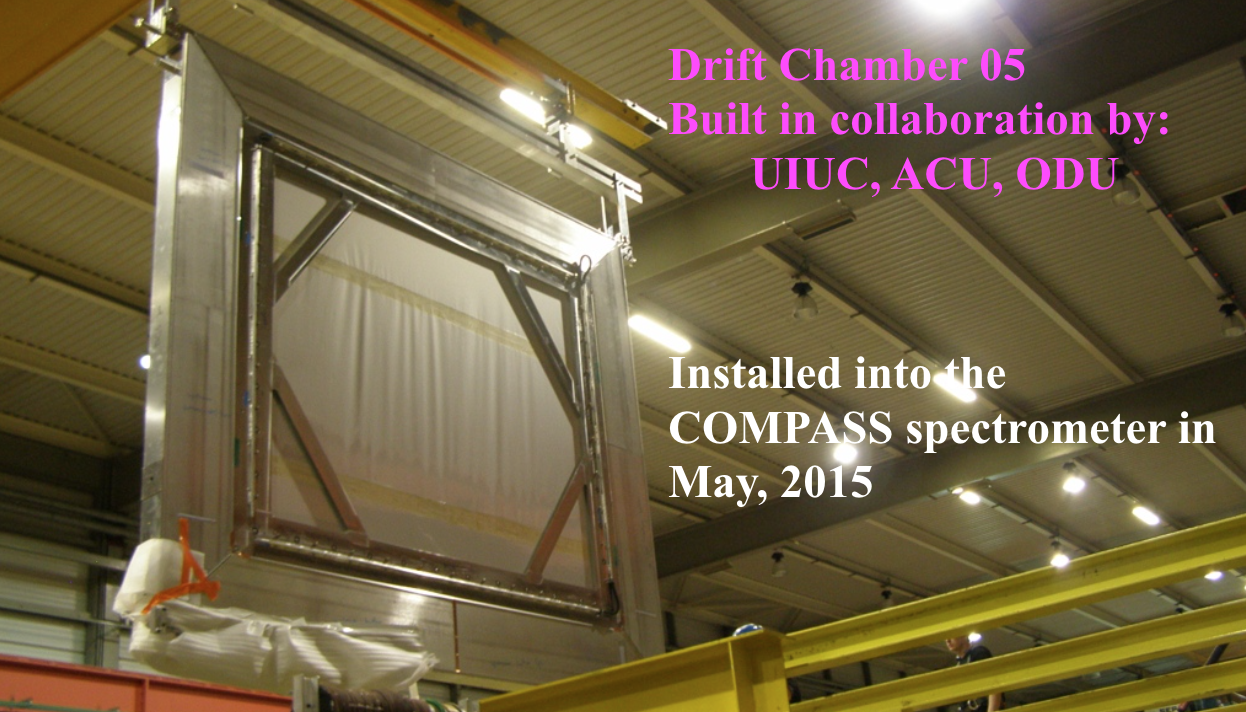
\includegraphics[width=0.5\textwidth]{DC05_full.png}
  \caption{}{The completed DC05 being craned into the COMPASS large area spectrometer.}
  \label{fig:DC05}%
\end{figure}

The design of DC05, figure~\ref{fig:DC05}, was based off a
previous large-area tracker at COMPASS.  DC05 has an
active area of 249x209cm$^2$ and consists of eight planes with a total
of 2304 sense wires and 2312 field wires.  The eight planes of DC05
correspond to four views, where each view measures a coordinate.  The
coordinates measured from DC05 are the horizontal, vertical and $\pm$
10$^{\circ}$ with respect to the horizontal.  The horizontal and
vertical coordinates consist of 2x256 sense wires and the offset to
horizontal coordinates each consist of 2x320 wires for increased
acceptance.  Each plane was made from a G-10 frame and five
frames stacked together constituting a view.  The whole detector was
closed in with two precision, stainless steel stiffening frames, which
were assembled with aluminized mylar as a gas window. \par The views
of DC05 consisted of three cathode layers and two anode
layers.  The cathodes layers were made from carbon paint sprayed on a
25 $\mu$m thin mylar layer.  There were two single-layer cathodes
layers and one layer with carbon on two sides within each view.
Additionally a 30 cm circular so-called beam killer was added to the cathodes to
control the efficiency in the central part of the detector.  The
cathodes were nominally set to -1675 V and the beam killer voltage was
set to -900 V for zero efficiency in the high flux central region.
The voltage on the beam killer can however be raised above the amplification threshold if the beam
flux is reduced and it is desirable to study the central region.  \par
The anode layers were made from alternating 20 $\mu$m gold-plated
tungsten sense wires and 100 $\mu$m gold-plated copper beryllium field
wires, as shown in figure~\ref{fig:driftcell}.  The field wires were
also placed at -1675 V and the sense wires were at 0 V.  The gas used
was made of: 45\% argon, for amplification; 45\% ethane, for
quenching; and 10\% CF$_4$, to reduce aging effects.  All these
properties corresponded to a gain of approximately 10$^4$.

\begin{figure}
  \centering
  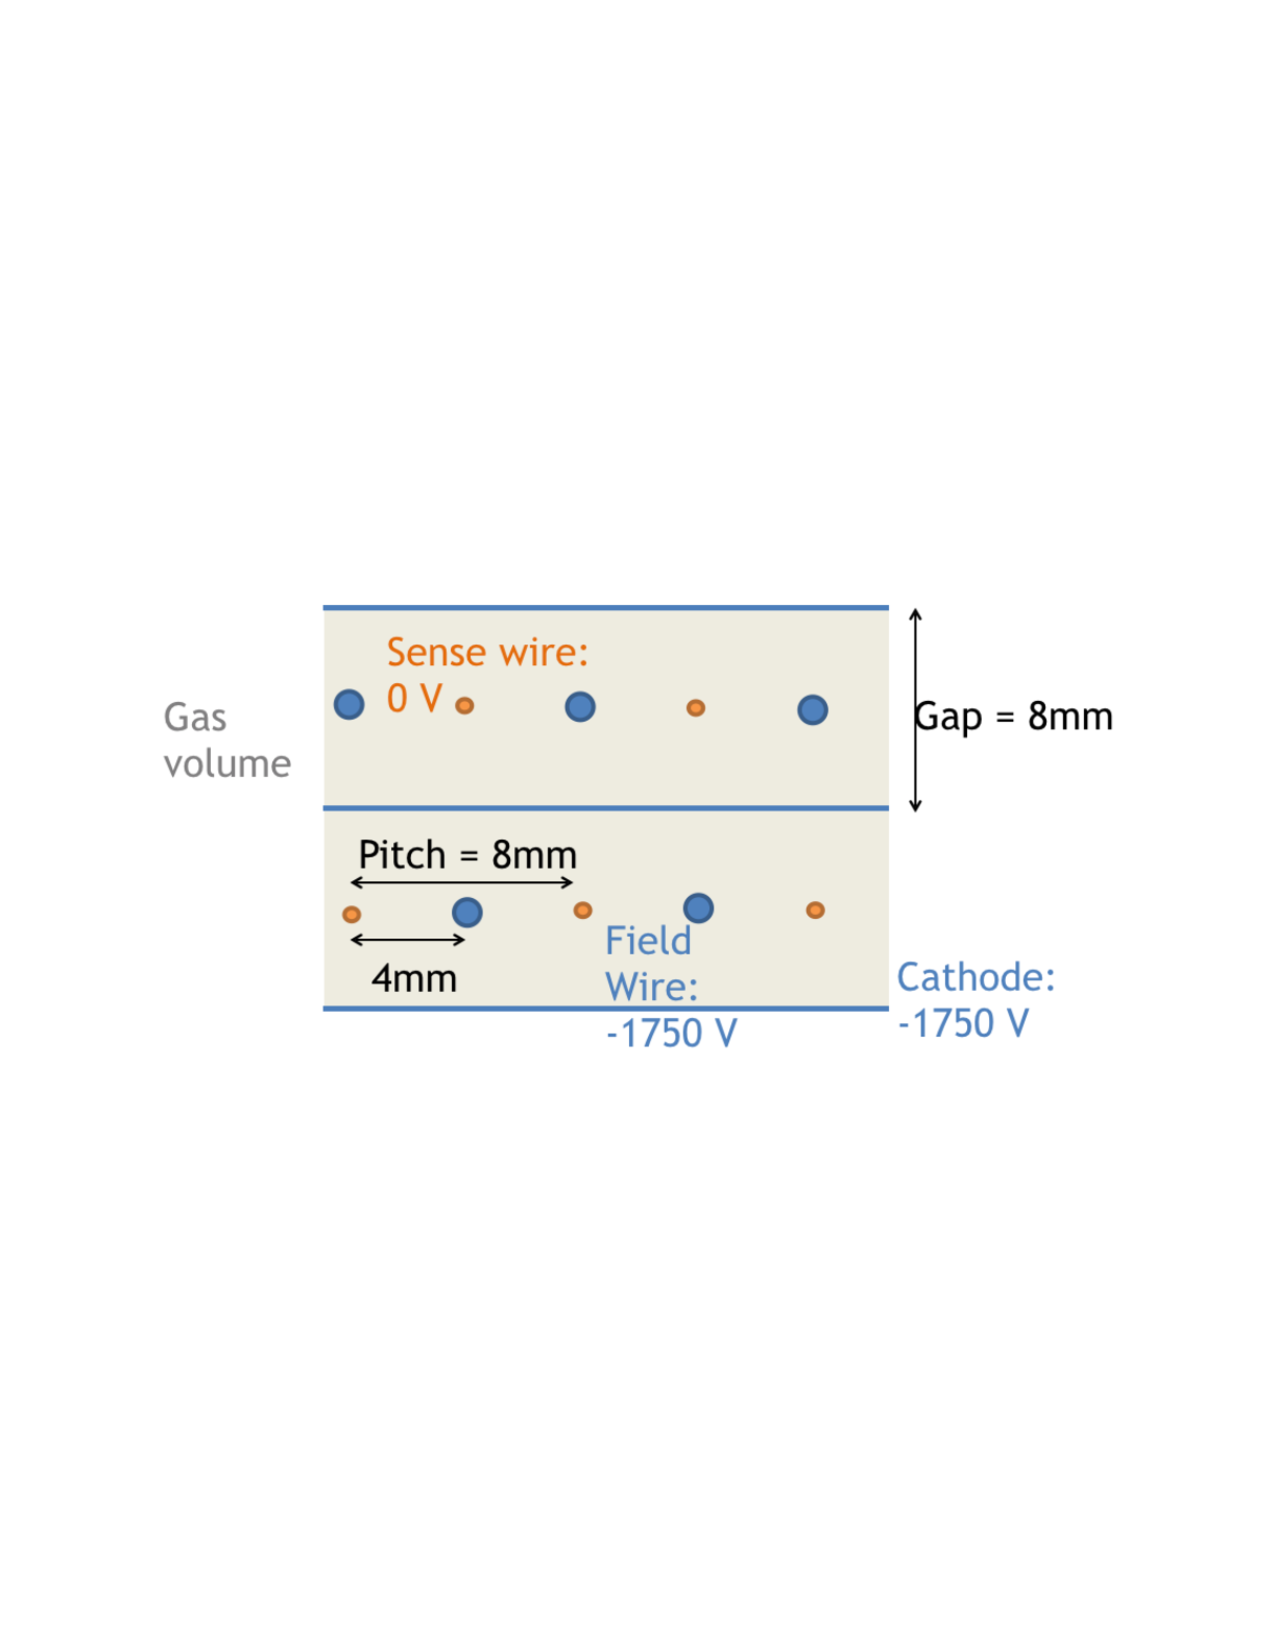
\includegraphics[width=0.5\textwidth]{DriftCell.png}
  \caption{}{The drift cell dimensions of one view in DC05.}
  \label{fig:driftcell}%
\end{figure}

\subsection{Construction}
The construction of DC05 was carried out as precisely as possible starting with the
precision from the stainless steel stiffening frames.  The stiffening frames
where cut with the highest relative accuracy by cutting the two frames on top of
each other to a precision of 50 $\mu$m everywhere in their plane.  The precision
from the stiffening frames was then transferred to the anode and cathode frames
through 40 positioning pins.  The G-10 frames were milled from strips at the NPL
using a precision milling machine.  Each four strips were then epoxied together
on top of one of the stiffening frames.  \par The cathodes had mylar stretched
and epoxied to them using a custom built stretching machine at CERN.  An
external company then spray painted carbon on them to make a resistance of
approximately 30 $k\Omega /m$.  All the sense and field wires were hand soldered
and subsequently verified for position using a microscope.  It was estimated the
position placement of each sense wire was at least as good as half the diameter
of a sense wire or precise to 10 $\mu$m.  The final assemble was done at CERN.
This consisted of stacking each of the 21 G-10 frames on top of the stiffening
frame and attaching copper electronic shielding all along the exterior of the
detector to reduce electronic noise. \par There were various tests performed
throughout the construction process for quality assurance before the final
installation.  The starting tests were measuring thickness and position of
important cuts on the G-10 strips using a micrometer.  G-10 strip thicknesses
were iteratively milled until they reached better than 50 $\mu$m in thickness
accuracy.  The thickness deviation of the whole detector including the stainless
steel stiffening frames was better than 750 $\mu$m.  The mechanical tension of the sense
wires was tested for stability by ensuring the voltage difference between sense
and field wires could reach as high as 2400 V in air.  In addition the wire
tension was cross-checked by determining the resonance frequency with which the
wires vibrated.  The resonance frequency was determined by placing the wires in
a constant magnetic field and varying a sinusoidal current across each wire till
the wires vibrated maximally.  The leakage current between sense and field wires
was verified to be less than 100 nA at nominal voltage in air.  Finally
amplification tests were first performed using a strontium-90 source and
verifying the counts per electronics board increased below the radioactive source.

\subsection{2015 Performance}
The overall performance of DC05 was checked using the COMPASS
reconstruction software CORAL.  In all cases the view of study was excluded from
the reconstruction algorithm and the individual hit information for the view of
interest was saved to get an unbiased measurement.  The efficiency was found to
be between 85\% and 90\% depending on the plane.  Using the so called RT
relation, figure~\ref{fig:RT}, the location of a track within a drift cell can
be most accurately determined.  This RT relation needs to be tuned as a
calibration to minimize the track residuals.  The RT relation also varies
depending on the beam type, intensity and the trigger type.  \par The double
layer residual was used to determine the position resolution.  The double layer
residual is the radial difference between the expected x/y positions of the two
planes in a view.  This double layer residual is independent of the track
resolution and only depends on the variance addition of the two individual
planes.  For the 2015 Drell-Yan physics taking the resolution achieved was
approximately 430 $\mu$m. This was determined by fitting the double residual with a
Gaussian to extract the variance and assumed equal variance per plane in a view.

\begin{figure}
  \centering 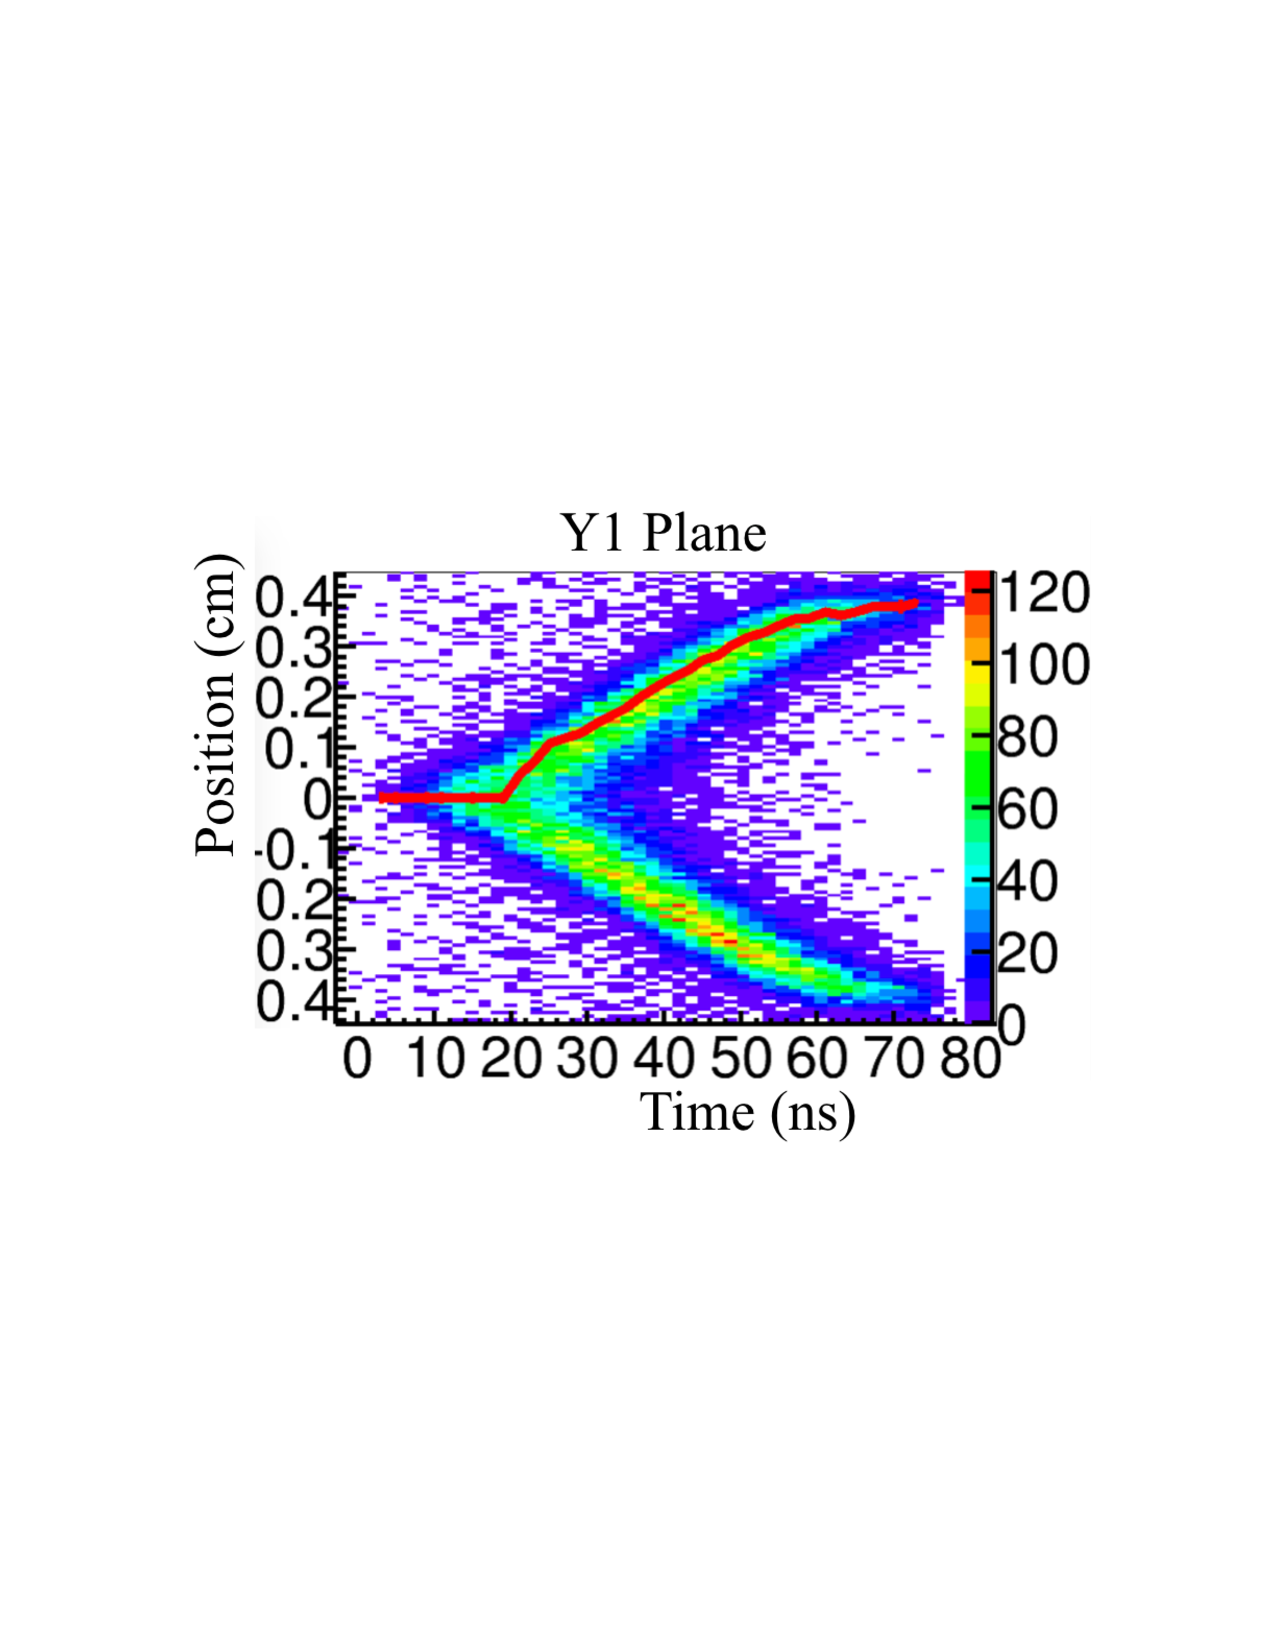
\includegraphics[width=0.5\textwidth]{RT_DC05Y2.png}
  \caption{}{Time versus position relation, or RT relation, after calibrating.
    The red fit shows the calibration determined.}
  \label{fig:RT}%
\end{figure}

\subsection{Conclusion}
The large-area DC05 was constructed at Illinois, Old Dominion University and
CERN.  It was built to upgrade the spectrometer performance at COMPASS and over
its two year construction period, involved the colaboration from students,
technicians and professors from five continents.  DC05 is a stable detector that
has been in use for two years and will continue to collect useful data for
future physics data taking at COMPASS.

% Put \label in argument of \section for cross-referencing
%\section{\label{}}
\subsection{}
\subsubsection{}

% If in two-column mode, this environment will change to single-column
% format so that long equations can be displayed. Use
% sparingly.
%\begin{widetext}
% put long equation here
%\end{widetext}

% figures should be put into the text as floats.
% Use the graphics or graphicx packages (distributed with LaTeX2e)
% and the \includegraphics macro defined in those packages.
% See the LaTeX Graphics Companion by Michel Goosens, Sebastian Rahtz,
% and Frank Mittelbach for instance.
%
% Here is an example of the general form of a figure:
% Fill in the caption in the braces of the \caption{} command. Put the label
% that you will use with \ref{} command in the braces of the \label{} command.
% Use the figure* environment if the figure should span across the
% entire page. There is no need to do explicit centering.

% \begin{figure}
% \includegraphics{}%
% \caption{\label{}}
% \end{figure}

% Surround figure environment with turnpage environment for landscape
% figure
% \begin{turnpage}
% \begin{figure}
% \includegraphics{}%
% \caption{\label{}}
% \end{figure}
% \end{turnpage}

% tables should appear as floats within the text
%
% Here is an example of the general form of a table:
% Fill in the caption in the braces of the \caption{} command. Put the label
% that you will use with \ref{} command in the braces of the \label{} command.
% Insert the column specifiers (l, r, c, d, etc.) in the empty braces of the
% \begin{tabular}{} command.
% The ruledtabular enviroment adds doubled rules to table and sets a
% reasonable default table settings.
% Use the table* environment to get a full-width table in two-column
% Add \usepackage{longtable} and the longtable (or longtable*}
% environment for nicely formatted long tables. Or use the the [H]
% placement option to break a long table (with less control than 
% in longtable).
% \begin{table}%[H] add [H] placement to break table across pages
% \caption{\label{}}
% \begin{ruledtabular}
% \begin{tabular}{}
% Lines of table here ending with \\
% \end{tabular}
% \end{ruledtabular}
% \end{table}

% Surround table environment with turnpage environment for landscape
% table
% \begin{turnpage}
% \begin{table}
% \caption{\label{}}
% \begin{ruledtabular}
% \begin{tabular}{}
% \end{tabular}
% \end{ruledtabular}
% \end{table}
% \end{turnpage}

% Specify following sections are appendices. Use \appendix* if there
% only one appendix.
%\appendix
%\section{}

% If you have acknowledgments, this puts in the proper section head.
%\begin{acknowledgments}
% put your acknowledgments here.
%\end{acknowledgments}

% Create the reference section using BibTeX:
%\bibliography{DC05.bib}
%\bibliography{DC05}
%\bibliography{test}
\input{DC05_bib.tex}

%\begin{thebibliography}{9}
%\bibitem{collins_2002} M.~Greene, J.~Schwarz, and
%E.~Witten, \textit{Superstring Theory:
%Introduction}, (Cambridge University
%Press, London, 1985).
%\end{thebibliography}

\end{document}
%
% ****** End of file apstemplate.tex ******

